\documentclass[]{article}
\usepackage{lmodern}
\usepackage{amssymb,amsmath}
\usepackage{ifxetex,ifluatex}
\usepackage{fixltx2e} % provides \textsubscript
\ifnum 0\ifxetex 1\fi\ifluatex 1\fi=0 % if pdftex
  \usepackage[T1]{fontenc}
  \usepackage[utf8]{inputenc}
\else % if luatex or xelatex
  \ifxetex
    \usepackage{mathspec}
  \else
    \usepackage{fontspec}
  \fi
  \defaultfontfeatures{Ligatures=TeX,Scale=MatchLowercase}
\fi
% use upquote if available, for straight quotes in verbatim environments
\IfFileExists{upquote.sty}{\usepackage{upquote}}{}
% use microtype if available
\IfFileExists{microtype.sty}{%
\usepackage{microtype}
\UseMicrotypeSet[protrusion]{basicmath} % disable protrusion for tt fonts
}{}
\usepackage[margin=1in]{geometry}
\usepackage{hyperref}
\hypersetup{unicode=true,
            pdftitle={Provident Regressions},
            pdfauthor={Dario Trujano Ochoa},
            pdfborder={0 0 0},
            breaklinks=true}
\urlstyle{same}  % don't use monospace font for urls
\usepackage{color}
\usepackage{fancyvrb}
\newcommand{\VerbBar}{|}
\newcommand{\VERB}{\Verb[commandchars=\\\{\}]}
\DefineVerbatimEnvironment{Highlighting}{Verbatim}{commandchars=\\\{\}}
% Add ',fontsize=\small' for more characters per line
\usepackage{framed}
\definecolor{shadecolor}{RGB}{248,248,248}
\newenvironment{Shaded}{\begin{snugshade}}{\end{snugshade}}
\newcommand{\KeywordTok}[1]{\textcolor[rgb]{0.13,0.29,0.53}{\textbf{#1}}}
\newcommand{\DataTypeTok}[1]{\textcolor[rgb]{0.13,0.29,0.53}{#1}}
\newcommand{\DecValTok}[1]{\textcolor[rgb]{0.00,0.00,0.81}{#1}}
\newcommand{\BaseNTok}[1]{\textcolor[rgb]{0.00,0.00,0.81}{#1}}
\newcommand{\FloatTok}[1]{\textcolor[rgb]{0.00,0.00,0.81}{#1}}
\newcommand{\ConstantTok}[1]{\textcolor[rgb]{0.00,0.00,0.00}{#1}}
\newcommand{\CharTok}[1]{\textcolor[rgb]{0.31,0.60,0.02}{#1}}
\newcommand{\SpecialCharTok}[1]{\textcolor[rgb]{0.00,0.00,0.00}{#1}}
\newcommand{\StringTok}[1]{\textcolor[rgb]{0.31,0.60,0.02}{#1}}
\newcommand{\VerbatimStringTok}[1]{\textcolor[rgb]{0.31,0.60,0.02}{#1}}
\newcommand{\SpecialStringTok}[1]{\textcolor[rgb]{0.31,0.60,0.02}{#1}}
\newcommand{\ImportTok}[1]{#1}
\newcommand{\CommentTok}[1]{\textcolor[rgb]{0.56,0.35,0.01}{\textit{#1}}}
\newcommand{\DocumentationTok}[1]{\textcolor[rgb]{0.56,0.35,0.01}{\textbf{\textit{#1}}}}
\newcommand{\AnnotationTok}[1]{\textcolor[rgb]{0.56,0.35,0.01}{\textbf{\textit{#1}}}}
\newcommand{\CommentVarTok}[1]{\textcolor[rgb]{0.56,0.35,0.01}{\textbf{\textit{#1}}}}
\newcommand{\OtherTok}[1]{\textcolor[rgb]{0.56,0.35,0.01}{#1}}
\newcommand{\FunctionTok}[1]{\textcolor[rgb]{0.00,0.00,0.00}{#1}}
\newcommand{\VariableTok}[1]{\textcolor[rgb]{0.00,0.00,0.00}{#1}}
\newcommand{\ControlFlowTok}[1]{\textcolor[rgb]{0.13,0.29,0.53}{\textbf{#1}}}
\newcommand{\OperatorTok}[1]{\textcolor[rgb]{0.81,0.36,0.00}{\textbf{#1}}}
\newcommand{\BuiltInTok}[1]{#1}
\newcommand{\ExtensionTok}[1]{#1}
\newcommand{\PreprocessorTok}[1]{\textcolor[rgb]{0.56,0.35,0.01}{\textit{#1}}}
\newcommand{\AttributeTok}[1]{\textcolor[rgb]{0.77,0.63,0.00}{#1}}
\newcommand{\RegionMarkerTok}[1]{#1}
\newcommand{\InformationTok}[1]{\textcolor[rgb]{0.56,0.35,0.01}{\textbf{\textit{#1}}}}
\newcommand{\WarningTok}[1]{\textcolor[rgb]{0.56,0.35,0.01}{\textbf{\textit{#1}}}}
\newcommand{\AlertTok}[1]{\textcolor[rgb]{0.94,0.16,0.16}{#1}}
\newcommand{\ErrorTok}[1]{\textcolor[rgb]{0.64,0.00,0.00}{\textbf{#1}}}
\newcommand{\NormalTok}[1]{#1}
\usepackage{graphicx,grffile}
\makeatletter
\def\maxwidth{\ifdim\Gin@nat@width>\linewidth\linewidth\else\Gin@nat@width\fi}
\def\maxheight{\ifdim\Gin@nat@height>\textheight\textheight\else\Gin@nat@height\fi}
\makeatother
% Scale images if necessary, so that they will not overflow the page
% margins by default, and it is still possible to overwrite the defaults
% using explicit options in \includegraphics[width, height, ...]{}
\setkeys{Gin}{width=\maxwidth,height=\maxheight,keepaspectratio}
\IfFileExists{parskip.sty}{%
\usepackage{parskip}
}{% else
\setlength{\parindent}{0pt}
\setlength{\parskip}{6pt plus 2pt minus 1pt}
}
\setlength{\emergencystretch}{3em}  % prevent overfull lines
\providecommand{\tightlist}{%
  \setlength{\itemsep}{0pt}\setlength{\parskip}{0pt}}
\setcounter{secnumdepth}{0}
% Redefines (sub)paragraphs to behave more like sections
\ifx\paragraph\undefined\else
\let\oldparagraph\paragraph
\renewcommand{\paragraph}[1]{\oldparagraph{#1}\mbox{}}
\fi
\ifx\subparagraph\undefined\else
\let\oldsubparagraph\subparagraph
\renewcommand{\subparagraph}[1]{\oldsubparagraph{#1}\mbox{}}
\fi

%%% Use protect on footnotes to avoid problems with footnotes in titles
\let\rmarkdownfootnote\footnote%
\def\footnote{\protect\rmarkdownfootnote}

%%% Change title format to be more compact
\usepackage{titling}

% Create subtitle command for use in maketitle
\newcommand{\subtitle}[1]{
  \posttitle{
    \begin{center}\large#1\end{center}
    }
}

\setlength{\droptitle}{-2em}
  \title{Provident Regressions}
  \pretitle{\vspace{\droptitle}\centering\huge}
  \posttitle{\par}
  \author{Dario Trujano Ochoa}
  \preauthor{\centering\large\emph}
  \postauthor{\par}
  \predate{\centering\large\emph}
  \postdate{\par}
  \date{Enero 2018}


\begin{document}
\maketitle

\subsection{Data Base}\label{data-base}

I imported the data to R; then, I cleaned for the cases with missing
values and reconfigured some variables:

\begin{Shaded}
\begin{Highlighting}[]
\CommentTok{# implort with more data}
\NormalTok{ProvidentDF_complete<-}\StringTok{ }\KeywordTok{read.csv}\NormalTok{(}\StringTok{"Encuesta-EducacionFinancieraDario.csv"}\NormalTok{)}

\NormalTok{ProvidentDF_complete <-}\StringTok{ }\NormalTok{ProvidentDF_complete }\OperatorTok\StringTok{ }\KeywordTok{filter}\NormalTok{(Status}\OperatorTok{==}\StringTok{"Completa"}\NormalTok{) }\OperatorTok\StringTok{ }
\StringTok{  }\KeywordTok{filter}\NormalTok{(}\OperatorTok{!}\KeywordTok{is.na}\NormalTok{(p9_batepelota)) }\CommentTok{# question 9 and 12 have missing values}
\CommentTok{# measure grit as the average of the points made in each item}
\NormalTok{ProvidentGRIT <-}\StringTok{ }\KeywordTok{data.frame}\NormalTok{(}
\NormalTok{  ProvidentDF_complete}\OperatorTok{$}\NormalTok{X1..Los.proyectos.o.ideas.nuevas.me.distraen.de.proyectos.o.ideas.que.ten.a.desde.antes.,}
\NormalTok{  ProvidentDF_complete}\OperatorTok{$}\NormalTok{X2..Los..bstaculos.no.me.desaniman.,}
\NormalTok{  ProvidentDF_complete}\OperatorTok{$}\NormalTok{X3..Estuve.concentrado.en.una.idea.o.proyecto.por.un.corto.tiempo..pero.despu.s.perd..inter.s.,}
\NormalTok{  ProvidentDF_complete}\OperatorTok{$}\NormalTok{X4..Trabajo.duro.,}
\NormalTok{  ProvidentDF_complete}\OperatorTok{$}\NormalTok{X5..Con.frecuencia.me.propongo.un.objetivo..pero.luego.trato.de.cumplir.un.objetivo.diferente,}
\NormalTok{  ProvidentDF_complete}\OperatorTok{$}\NormalTok{X6..Me.resulta.dificil.mantener.mi.atenci.n.en.proyectos.que.duran.m.s.all..de.algunos.meses.en.terminar,}
\NormalTok{  ProvidentDF_complete}\OperatorTok{$}\NormalTok{X7..Soy.chambeador.a.)}
\NormalTok{ProvidentGRIT <-}\StringTok{ }\KeywordTok{apply}\NormalTok{(}\KeywordTok{substr}\NormalTok{(}\KeywordTok{apply}\NormalTok{(ProvidentGRIT, }\DataTypeTok{MARGIN =} \DecValTok{2}\NormalTok{,}\DataTypeTok{FUN =}\NormalTok{ as.character),}\DataTypeTok{start =} \DecValTok{1}\NormalTok{,}\DataTypeTok{stop =} \DecValTok{1}\NormalTok{),}\DataTypeTok{FUN =}\NormalTok{ as.numeric,}\DataTypeTok{MARGIN =} \DecValTok{2}\NormalTok{)}
\NormalTok{ProvidentGRIT[,}\KeywordTok{c}\NormalTok{(}\DecValTok{1}\NormalTok{,}\DecValTok{3}\NormalTok{,}\DecValTok{5}\NormalTok{,}\DecValTok{6}\NormalTok{)] <-}\StringTok{ }\OperatorTok{-}\NormalTok{ProvidentGRIT[,}\KeywordTok{c}\NormalTok{(}\DecValTok{1}\NormalTok{,}\DecValTok{3}\NormalTok{,}\DecValTok{5}\NormalTok{,}\DecValTok{6}\NormalTok{)] }\OperatorTok{+}\StringTok{ }\DecValTok{4}
\NormalTok{ProvidentDF_nna <-}\StringTok{ }\NormalTok{ProvidentDF_complete }\OperatorTok\StringTok{  }\CommentTok{# there is no missing values in this DF}
\StringTok{  }\KeywordTok{mutate}\NormalTok{(}\DataTypeTok{grit=}\KeywordTok{rowMeans}\NormalTok{(ProvidentGRIT)) }
\NormalTok{ProvidentDF_nna <-}\StringTok{ }\NormalTok{ProvidentDF_nna[}\OperatorTok{!}\KeywordTok{is.na}\NormalTok{(ProvidentDF_nna}\OperatorTok{$}\NormalTok{p9_batepelota),]}

\CommentTok{# Education}
\NormalTok{escol <-}\StringTok{ }\KeywordTok{as.character}\NormalTok{(ProvidentDF_nna}\OperatorTok{$}\NormalTok{escol)}
\NormalTok{escol[escol}\OperatorTok{==}\StringTok{"No estudi¢"}\NormalTok{] <-}\StringTok{ }\DecValTok{0}
\NormalTok{escol[escol}\OperatorTok{==}\StringTok{"1ro Primaria"}\NormalTok{] <-}\StringTok{ }\DecValTok{1}
\NormalTok{escol[escol}\OperatorTok{==}\StringTok{"2do Primaria"}\NormalTok{] <-}\StringTok{ }\DecValTok{2}
\NormalTok{escol[escol}\OperatorTok{==}\StringTok{"3ro Primaria"}\NormalTok{] <-}\StringTok{ }\DecValTok{3}
\NormalTok{escol[escol}\OperatorTok\KeywordTok{c}\NormalTok{(}\StringTok{"4to primaria"}\NormalTok{,}\StringTok{"4to Primaria"}\NormalTok{)] <-}\StringTok{ }\DecValTok{4}
\NormalTok{escol[escol}\OperatorTok{==}\StringTok{"5to Primaria"}\NormalTok{] <-}\StringTok{ }\DecValTok{5}
\NormalTok{escol[escol}\OperatorTok\KeywordTok{c}\NormalTok{(}\StringTok{" 6to Primaria"}\NormalTok{,}\StringTok{"6to Primaria"}\NormalTok{)] <-}\StringTok{ }\DecValTok{6}
\NormalTok{escol[escol}\OperatorTok{==}\StringTok{"1ro Secundaria"}\NormalTok{] <-}\StringTok{ }\DecValTok{7}
\NormalTok{escol[escol}\OperatorTok\KeywordTok{c}\NormalTok{(}\StringTok{"2do Secundaria"}\NormalTok{,}\StringTok{"2do secundaria"}\NormalTok{)] <-}\StringTok{ }\DecValTok{8}
\NormalTok{escol[escol}\OperatorTok\KeywordTok{c}\NormalTok{(}\StringTok{"3ro secundaria"}\NormalTok{,}\StringTok{"3ro Secundaria "}\NormalTok{,}\StringTok{"3ro Secundaria"}\NormalTok{)] <-}\StringTok{ }\DecValTok{9}
\NormalTok{escol[escol}\OperatorTok{==}\StringTok{"1ro Preparatoria"}\NormalTok{] <-}\StringTok{ }\DecValTok{10}
\NormalTok{escol[escol}\OperatorTok{==}\StringTok{"2do Preparatoria"}\NormalTok{] <-}\StringTok{ }\DecValTok{11}
\NormalTok{escol[escol}\OperatorTok{==}\StringTok{"3ro Preparatoria"}\NormalTok{] <-}\StringTok{ }\DecValTok{12}
\NormalTok{escol[escol}\OperatorTok{==}\StringTok{"Licenciatura"}\NormalTok{] <-}\StringTok{ }\DecValTok{13}
\NormalTok{escol[escol}\OperatorTok{==}\StringTok{"Posgrado"}\NormalTok{] <-}\StringTok{ }\DecValTok{14}
\NormalTok{escol <-}\StringTok{ }\KeywordTok{as.numeric}\NormalTok{(escol)}

\CommentTok{#original measure}
\NormalTok{escol1 <-}\StringTok{ }\NormalTok{escol}
\NormalTok{escol1[escol1}\OperatorTok\KeywordTok{c}\NormalTok{(}\DecValTok{1}\OperatorTok{:}\DecValTok{6}\NormalTok{)]<-}\StringTok{ }\DecValTok{0} \CommentTok{# Primaria}
\NormalTok{escol1[escol1}\OperatorTok\KeywordTok{c}\NormalTok{(}\DecValTok{7}\OperatorTok{:}\DecValTok{9}\NormalTok{)]<-}\StringTok{ }\DecValTok{1} \CommentTok{# Secundaria}
\NormalTok{escol1[escol1}\OperatorTok\KeywordTok{c}\NormalTok{(}\DecValTok{10}\OperatorTok{:}\DecValTok{12}\NormalTok{)]<-}\StringTok{ }\DecValTok{2} \CommentTok{# Preparatoria}
\NormalTok{escol1[escol1}\OperatorTok\KeywordTok{c}\NormalTok{(}\DecValTok{13}\NormalTok{)]<-}\StringTok{ }\DecValTok{3} \CommentTok{# Licenciatura}
\NormalTok{escol1[escol1}\OperatorTok\KeywordTok{c}\NormalTok{(}\DecValTok{14}\NormalTok{)]<-}\StringTok{ }\DecValTok{4} \CommentTok{# Posgrado}



\CommentTok{#some order for ordinal data}
\NormalTok{ProvidentDF_nna}\OperatorTok{$}\NormalTok{grupo <-}\StringTok{ }\KeywordTok{factor}\NormalTok{(ProvidentDF_nna}\OperatorTok{$}\NormalTok{grupo, }\DataTypeTok{levels=}\KeywordTok{c}\NormalTok{(}\StringTok{"Current"}\NormalTok{, }\StringTok{"Low Arrear"}\NormalTok{,}\StringTok{"High arrear"}\NormalTok{), }\DataTypeTok{ordered=}\OtherTok{TRUE}\NormalTok{)}

\KeywordTok{attach}\NormalTok{(ProvidentDF_nna)}
\end{Highlighting}
\end{Shaded}

\begin{verbatim}
## The following object is masked _by_ .GlobalEnv:
## 
##     escol
\end{verbatim}

\begin{itemize}
\item
  Just married and not married
\item
  Married = 1
\item
  Employment as an ordinal variable.
\item
  Full-time employment = 3
\item
  Half-time employment = 2
\item
  Self-employment = 1
\item
  No earnings = 0
\end{itemize}

\begin{Shaded}
\begin{Highlighting}[]
\NormalTok{p16_dependents<-}\StringTok{ }\NormalTok{p16_1menores}\OperatorTok{+}\NormalTok{p16_2adulmay}\OperatorTok{+}\NormalTok{p16_3otros }\CommentTok{# total number of dependents}
\NormalTok{casado<-\{\} }\CommentTok{# to capture later de degree of responsability, we just need married or unmarried people}
\NormalTok{casado[p15_estadocivil}\OperatorTok{==}\StringTok{"Casado"}\NormalTok{]<-}\StringTok{ }\DecValTok{1}
\NormalTok{casado[p15_estadocivil}\OperatorTok{!=}\StringTok{"Casado"}\NormalTok{]<-}\StringTok{ }\DecValTok{0}
\NormalTok{empleoRemunerado <-}\StringTok{ }\NormalTok{\{\} }\CommentTok{# consider non paid work together }
\NormalTok{empleoRemunerado[statusempleo}\OperatorTok\KeywordTok{c}\NormalTok{(}\StringTok{"Desempleados"}\NormalTok{,}\StringTok{"Ama de Casa"}\NormalTok{,}\StringTok{"Retirado"}\NormalTok{)]<-}\StringTok{ }\DecValTok{0}
\NormalTok{empleoRemunerado[statusempleo}\OperatorTok{==}\StringTok{"Auto empleado"}\NormalTok{]<-}\StringTok{ }\DecValTok{1}
\NormalTok{empleoRemunerado[statusempleo}\OperatorTok{==}\StringTok{"Empleado Medio tiempo"}\NormalTok{]<-}\StringTok{ }\DecValTok{2}
\NormalTok{empleoRemunerado[statusempleo}\OperatorTok{==}\StringTok{"Empleado tiempo completo"}\NormalTok{]<-}\StringTok{ }\DecValTok{3}
\end{Highlighting}
\end{Shaded}

\begin{itemize}
\tightlist
\item
  To masure the responses in the Finantial literacy we take the distance
  from the correct answers:
\end{itemize}

\begin{Shaded}
\begin{Highlighting}[]
\CommentTok{# pregunta del bat y la pelota:}
\CommentTok{# We can see that most people answered predictably bad: $ 10. But no one answered correctly.}
\KeywordTok{barplot}\NormalTok{(}\KeywordTok{table}\NormalTok{(p9_batepelota))}
\end{Highlighting}
\end{Shaded}

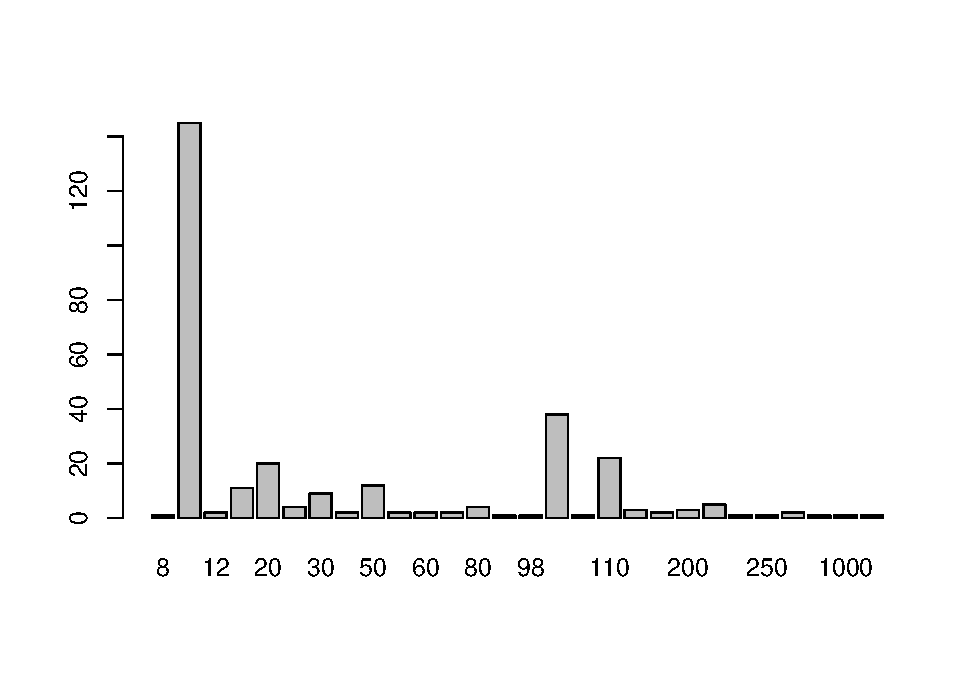
\includegraphics{ProvidentRegressions_files/figure-latex/unnamed-chunk-3-1.pdf}

\begin{Shaded}
\begin{Highlighting}[]
\CommentTok{#9. Un bate y una pelota de béisbol cuestan en total $110 pesos. }
\CommentTok{#El bate cuesta $100 más que la pelota, }
\CommentTok{#¿Cuánto cuesta la pelota? (Indique el costo en pesos de la pelota)}
\NormalTok{## Respuesta correcta: $5}

\NormalTok{p9_batepelota<-}\StringTok{ }\KeywordTok{abs}\NormalTok{(p9_batepelota}\OperatorTok{-}\DecValTok{5}\NormalTok{)}

\CommentTok{# pregunta sobre el Interés}
\KeywordTok{barplot}\NormalTok{(}\KeywordTok{table}\NormalTok{(p12_retornodeposito))}
\end{Highlighting}
\end{Shaded}

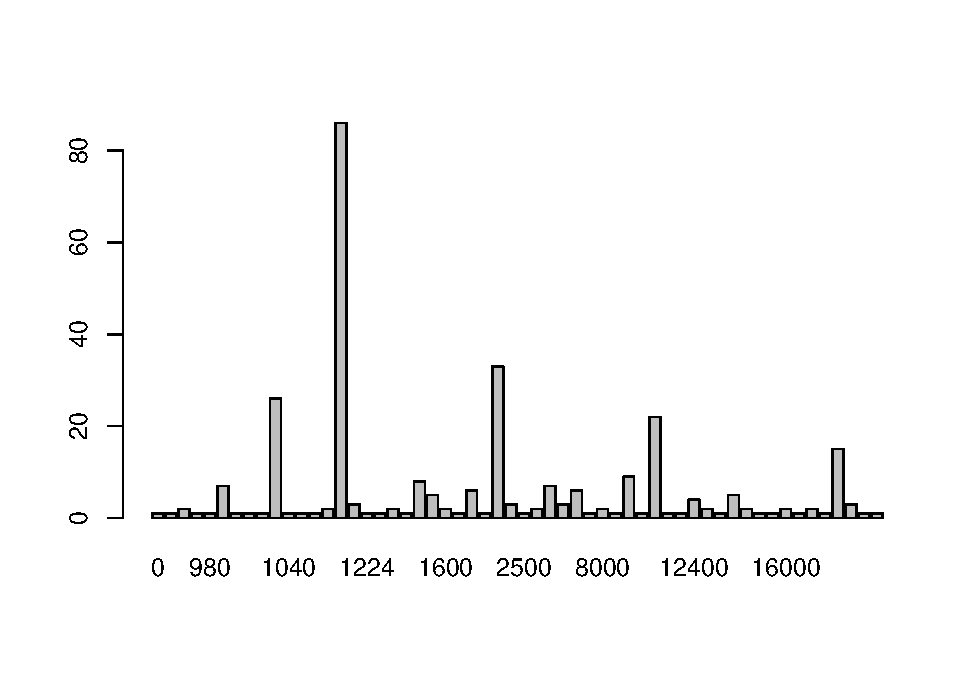
\includegraphics{ProvidentRegressions_files/figure-latex/unnamed-chunk-3-2.pdf}

\begin{Shaded}
\begin{Highlighting}[]
\CommentTok{#12. Imagínese que usted deposita $1,000 pesos al inicio del año en una cuenta de ahorro }
\CommentTok{#con un interés garantizado del 2% al año y la cuenta no tiene ningún costo por mantenerla. }
\CommentTok{#Además, suponga que usted no saca dinero de esa cuenta.}
\CommentTok{#¿Cuánto dinero tendría en la cuenta después de un año incluyendo el pago de los intereses?}
\NormalTok{## Respuesta Correcta: 1020}
\NormalTok{p12_retornodeposito <-}\StringTok{ }\KeywordTok{abs}\NormalTok{(p12_retornodeposito}\OperatorTok{-}\DecValTok{1020}\NormalTok{)}
\end{Highlighting}
\end{Shaded}

\subsection{PCA analysis}\label{pca-analysis}

First of all I have to highlight that there is an important error in the
way indeces were constructed in the article: eigenvalues were calculated
using no centered data which lead towards a biased estimate of the
index. In this case the variable with the hights mena will attract all
the weight.

Considering that all the regression made over the those indices are
wrong.

I'll consider the ideces as constructed in the article:

\begin{Shaded}
\begin{Highlighting}[]
\CommentTok{# time preference}
\NormalTok{TP <-}\StringTok{ }\KeywordTok{prcomp}\NormalTok{(}\KeywordTok{na.omit}\NormalTok{(}\KeywordTok{cbind}\NormalTok{(p10_tandacorto,p11_tandalargo)),}\DataTypeTok{center =}\NormalTok{ T,}\DataTypeTok{scale. =}\NormalTok{ T)}
\CommentTok{#cognitive hability}
\NormalTok{CA <-}\StringTok{ }\KeywordTok{prcomp}\NormalTok{(}\KeywordTok{na.omit}\NormalTok{(}\KeywordTok{cbind}\NormalTok{( p9_batepelota, p12_retornodeposito,p13_preciosbajan,escol)),}\DataTypeTok{center =}\NormalTok{ T,}\DataTypeTok{scale. =}\NormalTok{ T) }\CommentTok{# For p13, "VERDADERO" was considered as 1 (TRUE)}
\CommentTok{# cognitive ability with less levels for escol}
\NormalTok{CA1 <-}\StringTok{ }\KeywordTok{prcomp}\NormalTok{(}\KeywordTok{na.omit}\NormalTok{(}\KeywordTok{cbind}\NormalTok{( p9_batepelota, p12_retornodeposito,p13_preciosbajan,escol1)),}\DataTypeTok{center =}\NormalTok{ T,}\DataTypeTok{scale. =}\NormalTok{ T)}
\CommentTok{# responsability}
\NormalTok{RES <-}\StringTok{ }\KeywordTok{prcomp}\NormalTok{(}\KeywordTok{na.omit}\NormalTok{(}\KeywordTok{cbind}\NormalTok{(edad,hijos,casado, p16_dependents)),}\DataTypeTok{center =}\NormalTok{ T,}\DataTypeTok{scale. =}\NormalTok{ T)}
\CommentTok{# economic sucess}
\NormalTok{ES <-}\StringTok{ }\KeywordTok{prcomp}\NormalTok{(}\KeywordTok{na.omit}\NormalTok{(}\KeywordTok{cbind}\NormalTok{(empleoRemunerado,SCelular,STelCasa,SResidencia)),}\DataTypeTok{center =}\NormalTok{ T,}\DataTypeTok{scale. =}\NormalTok{ T)}
\end{Highlighting}
\end{Shaded}

PCA visual analysis shows that there is no a big difference in the
variance explained by the components:

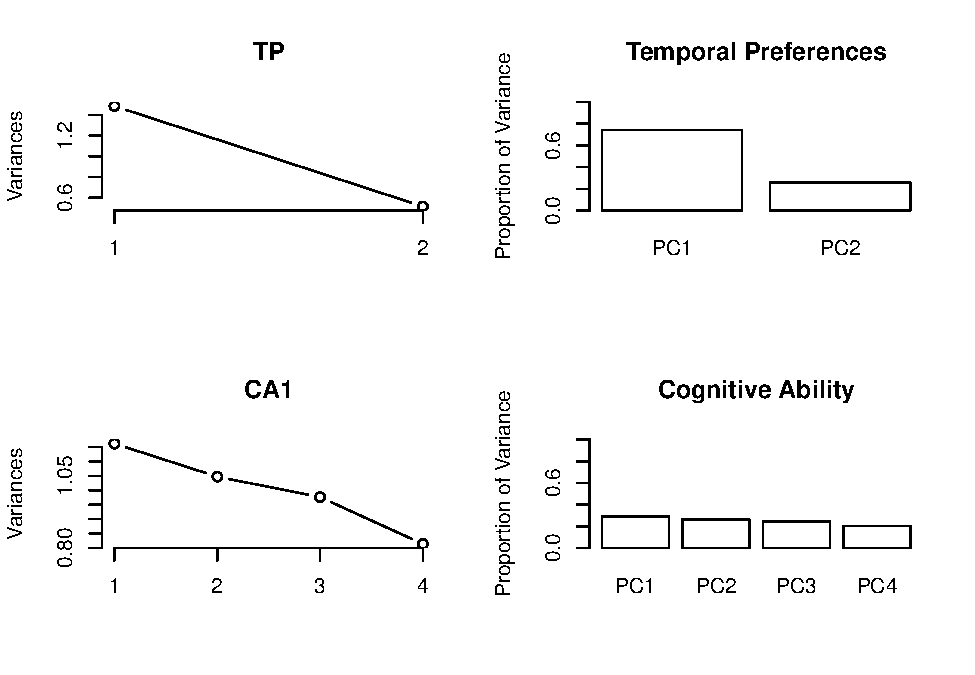
\includegraphics{ProvidentRegressions_files/figure-latex/unnamed-chunk-5-1.pdf}

\subsubsection{PCA weigths}\label{pca-weigths}

\begin{Shaded}
\begin{Highlighting}[]
\NormalTok{TP}\OperatorTok{$}\NormalTok{rotation}
\end{Highlighting}
\end{Shaded}

\begin{verbatim}
##                      PC1        PC2
## p10_tandacorto 0.7071068  0.7071068
## p11_tandalargo 0.7071068 -0.7071068
\end{verbatim}

\begin{Shaded}
\begin{Highlighting}[]
\NormalTok{CA}\OperatorTok{$}\NormalTok{rotation}
\end{Highlighting}
\end{Shaded}

\begin{verbatim}
##                            PC1          PC2         PC3        PC4
## p9_batepelota       -0.1725868  0.692953358 -0.63869914 -0.2865185
## p12_retornodeposito -0.1795121  0.622998104  0.75772040 -0.0742197
## p13_preciosbajan    -0.6510778 -0.362828070  0.07923137 -0.6619485
## escol                0.7169985 -0.006693184  0.10791477 -0.6886383
\end{verbatim}

\begin{Shaded}
\begin{Highlighting}[]
\NormalTok{RES}\OperatorTok{$}\NormalTok{rotation}
\end{Highlighting}
\end{Shaded}

\begin{verbatim}
##                       PC1         PC2        PC3         PC4
## edad           -0.3751918  0.64613531 -0.5833343  0.31853004
## hijos           0.5919374  0.19803781 -0.4925299 -0.60646964
## casado          0.2569157  0.73105085  0.6316692 -0.02351686
## p16_dependents  0.6654589 -0.09410012 -0.1346455  0.72813470
\end{verbatim}

\begin{Shaded}
\begin{Highlighting}[]
\NormalTok{ES}\OperatorTok{$}\NormalTok{rotation}
\end{Highlighting}
\end{Shaded}

\begin{verbatim}
##                         PC1        PC2          PC3       PC4
## empleoRemunerado  0.3109411 -0.3418428  0.876328114 0.1360446
## SCelular          0.6481033  0.1812993 -0.266362713 0.6900316
## STelCasa         -0.6436841 -0.3333109 -0.008564225 0.6888405
## SResidencia      -0.2625804  0.8597545  0.401281193 0.1756334
\end{verbatim}

\subsection{Final Regressions with
PCA}\label{final-regressions-with-pca}

\begin{Shaded}
\begin{Highlighting}[]
\NormalTok{DV <-}\StringTok{ }\KeywordTok{cbind.data.frame}\NormalTok{(}
       \DataTypeTok{Grit =}\NormalTok{ grit,}
       \DataTypeTok{TP1 =}\NormalTok{ TP}\OperatorTok{$}\NormalTok{x[,}\DecValTok{1}\NormalTok{], }\DataTypeTok{TP2 =}\NormalTok{ TP}\OperatorTok{$}\NormalTok{x[,}\DecValTok{2}\NormalTok{],}
       \DataTypeTok{CA1 =}\NormalTok{ CA1}\OperatorTok{$}\NormalTok{x[,}\DecValTok{1}\NormalTok{], }\DataTypeTok{CA2 =}\NormalTok{ CA1}\OperatorTok{$}\NormalTok{x[,}\DecValTok{2}\NormalTok{],}
       \DataTypeTok{ES1 =}\NormalTok{ ES}\OperatorTok{$}\NormalTok{x[,}\DecValTok{1}\NormalTok{], }\DataTypeTok{ES2 =}\NormalTok{ ES}\OperatorTok{$}\NormalTok{x[,}\DecValTok{2}\NormalTok{],}
\NormalTok{       edad, hijos,casado, p16_dependents,}
\NormalTok{       ProvidentDF_nna}\OperatorTok{$}\NormalTok{Prestamos.activos,}
\NormalTok{       Genero)}

\NormalTok{final_regression <-}\StringTok{ }\KeywordTok{polr}\NormalTok{(grupo }\OperatorTok{~}\StringTok{ }\NormalTok{Grit}\OperatorTok{+}\NormalTok{TP2}\OperatorTok{+}\NormalTok{CA2}\OperatorTok{+}\NormalTok{edad, }\DataTypeTok{data =}\NormalTok{ DV,}\DataTypeTok{Hess=}\OtherTok{TRUE}\NormalTok{,}\DataTypeTok{na.action =}\NormalTok{ na.omit) }\CommentTok{# model}
  \KeywordTok{stargazer}\NormalTok{(final_regression)}
\end{Highlighting}
\end{Shaded}

\% Table created by stargazer v.5.2 by Marek Hlavac, Harvard University.
E-mail: hlavac at fas.harvard.edu \% Date and time: lun., ene. 15, 2018
- 09:30:28 p.~m.

\begin{table}[!htbp] \centering 
  \caption{} 
  \label{} 
\begin{tabular}{@{\extracolsep{5pt}}lc} 
\\[-1.8ex]\hline 
\hline \\[-1.8ex] 
 & \multicolumn{1}{c}{\textit{Dependent variable:}} \\ 
\cline{2-2} 
\\[-1.8ex] & grupo \\ 
\hline \\[-1.8ex] 
 Grit & $-$0.503$^{**}$ \\ 
  & (0.241) \\ 
  & \\ 
 TP2 & 0.500$^{***}$ \\ 
  & (0.161) \\ 
  & \\ 
 CA2 & $-$0.213$^{*}$ \\ 
  & (0.116) \\ 
  & \\ 
 edad & $-$0.028$^{***}$ \\ 
  & (0.009) \\ 
  & \\ 
\hline \\[-1.8ex] 
Observations & 299 \\ 
\hline 
\hline \\[-1.8ex] 
\textit{Note:}  & \multicolumn{1}{r}{$^{*}$p$<$0.1; $^{**}$p$<$0.05; $^{***}$p$<$0.01} \\ 
\end{tabular} 
\end{table}

In order to maintain the significance of CA2, it was required that escol
was constructed according with the first categorization, otherwise the
component is significative just at 10\%. It is remarkable that this
categorization consider no instruction and elementary instruction in the
same level of escolarity.

\paragraph{Robustez}\label{robustez}

\% Table created by stargazer v.5.2 by Marek Hlavac, Harvard University.
E-mail: hlavac at fas.harvard.edu \% Date and time: lun., ene. 15, 2018
- 09:30:33 p.~m.

\begin{table}[!htbp] \centering 
  \caption{} 
  \label{} 
\begin{tabular}{@{\extracolsep{5pt}}lccccccc} 
\\[-1.8ex]\hline 
\hline \\[-1.8ex] 
 & \multicolumn{7}{c}{\textit{Dependent variable:}} \\ 
\cline{2-8} 
\\[-1.8ex] & \multicolumn{7}{c}{grupo} \\ 
\\[-1.8ex] & (1) & (2) & (3) & (4) & (5) & (6) & (7)\\ 
\hline \\[-1.8ex] 
 Grit & $-$0.503$^{**}$ & $-$0.517$^{**}$ & $-$0.520$^{**}$ & $-$0.428$^{*}$ & $-$0.503$^{**}$ &  & $-$0.448$^{*}$ \\ 
  & (0.241) & (0.242) & (0.243) & (0.238) & (0.241) &  & (0.239) \\ 
  & & & & & & & \\ 
 TP1 &  & 0.132 & 0.127 &  &  & 0.125 & 0.113 \\ 
  &  & (0.087) & (0.087) &  &  & (0.086) & (0.086) \\ 
  & & & & & & & \\ 
 TP2 & 0.500$^{***}$ & 0.507$^{***}$ & 0.515$^{***}$ & 0.460$^{***}$ & 0.500$^{***}$ & 0.504$^{***}$ & 0.466$^{***}$ \\ 
  & (0.161) & (0.162) & (0.162) & (0.158) & (0.161) & (0.162) & (0.159) \\ 
  & & & & & & & \\ 
 CA2 & $-$0.213$^{*}$ & $-$0.231$^{**}$ & $-$0.239$^{**}$ & $-$0.210$^{*}$ & $-$0.213$^{*}$ & $-$0.198$^{*}$ &  \\ 
  & (0.116) & (0.116) & (0.117) & (0.115) & (0.116) & (0.114) &  \\ 
  & & & & & & & \\ 
 edad & $-$0.028$^{***}$ & $-$0.027$^{***}$ & $-$0.027$^{***}$ &  & $-$0.028$^{***}$ & $-$0.025$^{***}$ & $-$0.027$^{***}$ \\ 
  & (0.009) & (0.009) & (0.009) &  & (0.009) & (0.009) & (0.009) \\ 
  & & & & & & & \\ 
 casado &  &  & $-$0.155 &  &  &  &  \\ 
  &  &  & (0.220) &  &  &  &  \\ 
  & & & & & & & \\ 
\hline \\[-1.8ex] 
AIC & 645.35 & 645.04 & 646.54 & 653.02 & 645.35 & 647.65 & 647.37 \\ 
BIC & 667.55 & 670.94 & 676.14 & 671.52 & 667.55 & 669.86 & 669.57 \\ 
Observations & 299 & 299 & 299 & 299 & 299 & 299 & 299 \\ 
\hline 
\hline \\[-1.8ex] 
\textit{Note:}  & \multicolumn{7}{r}{$^{*}$p$<$0.1; $^{**}$p$<$0.05; $^{***}$p$<$0.01} \\ 
\end{tabular} 
\end{table}

\subsection{Considering debt history}\label{considering-debt-history}

\% Table created by stargazer v.5.2 by Marek Hlavac, Harvard University.
E-mail: hlavac at fas.harvard.edu \% Date and time: lun., ene. 15, 2018
- 09:30:33 p.~m.

\begin{table}[!htbp] \centering 
  \caption{} 
  \label{} 
\begin{tabular}{@{\extracolsep{5pt}}lccc} 
\\[-1.8ex]\hline 
\hline \\[-1.8ex] 
 & \multicolumn{3}{c}{\textit{Dependent variable:}} \\ 
\cline{2-4} 
\\[-1.8ex] & \multicolumn{3}{c}{grupo} \\ 
\\[-1.8ex] & (1) & (2) & (3)\\ 
\hline \\[-1.8ex] 
 Grit & $-$0.517$^{**}$ & $-$0.514$^{**}$ & $-$0.514$^{**}$ \\ 
  & (0.242) & (0.261) & (0.261) \\ 
  & & & \\ 
 TP1 & 0.132 & 0.121 &  \\ 
  & (0.087) & (0.092) &  \\ 
  & & & \\ 
 TP2 & 0.507$^{***}$ & 0.352$^{**}$ &  \\ 
  & (0.162) & (0.170) &  \\ 
  & & & \\ 
 p10\_tandacorto &  &  & 0.818$^{**}$ \\ 
  &  &  & (0.342) \\ 
  & & & \\ 
 p11\_tandalargo &  &  & $-$0.411 \\ 
  &  &  & (0.336) \\ 
  & & & \\ 
 CA2 & $-$0.231$^{**}$ & $-$0.194 & $-$0.194 \\ 
  & (0.116) & (0.124) & (0.124) \\ 
  & & & \\ 
 edad & $-$0.027$^{***}$ & $-$0.017$^{*}$ & $-$0.017$^{*}$ \\ 
  & (0.009) & (0.010) & (0.010) \\ 
  & & & \\ 
 Prestamos.activos &  & $-$1.744$^{***}$ & $-$1.744$^{***}$ \\ 
  &  & (0.222) & (0.222) \\ 
  & & & \\ 
\hline \\[-1.8ex] 
AIC & 645.04 & 573.36 & 573.36 \\ 
BIC & 670.94 & 602.96 & 602.96 \\ 
Observations & 299 & 299 & 299 \\ 
\hline 
\hline \\[-1.8ex] 
\textit{Note:}  & \multicolumn{3}{r}{$^{*}$p$<$0.1; $^{**}$p$<$0.05; $^{***}$p$<$0.01} \\ 
\end{tabular} 
\end{table}


\end{document}
